% Homework template for Inference and Information
% UPDATE: September 26, 2017 by Xiangxiang
\documentclass[a4paper]{article}
\usepackage{amsmath, amssymb, amsthm}
% amsmath: equation*, amssymb: mathbb, amsthm: proof
\usepackage{moreenum}
\usepackage{mathtools}
\usepackage{url}
\usepackage{enumitem}
\usepackage{graphicx}
\usepackage{subcaption}
\usepackage{booktabs} % toprule
\usepackage[mathcal]{eucal}
%% Definitions for Inference and Information
%% UPDATE: 22/03/2018  by zhaofeng-shu33
%% This package does not require other packages
\ProvidesPackage{dtx-style}
% semester
\newcommand{\theterm}[1]{#1}
\newcommand{\thecourseinstitute}[1]{#1}
\newcommand{\thecoursename}[1]{\textsc{#1}}

\newcommand{\courseheader}[3]{
\vspace*{-1in}
\begin{center}
\thecourseinstitute{#1}\\
\thecoursename{#3} \\
\theterm{#2}
\vspace*{0.1in}
\hrule
\end{center}
}
\def\v#1{\underline{#1}}
\newcommand{\rvx}{\mathsf{x}}    % x, r.v.
\newcommand{\rvy}{\mathsf{y}}    % y, r.v.
\newcommand{\rvz}{\mathsf{z}}    % z, r.v.
\newcommand{\rvH}{\mathsf{H}} 
\newcommand{\uy}{\underline{y}}
\newcommand{\urvx}{\underline{\mathsf{x}}}    % x, r.v. vec
\newcommand{\urvy}{\underline{\mathsf{y}}}    % y, r.v. vec
\newcommand{\urvz}{\underline{\mathsf{z}}}    % z, r.v. vec
\newcommand{\urvw}{\underline{\mathsf{w}}} 
\newcommand{\defas}{\triangleq} %\coloneqq
\newcommand{\reals}{\mathbb{R}}
\newcommand{\TT}{\mathrm{T}}    % transpose
% \newcommand{\E}[1]{\mathbb{E}\left[{#1}\right]}
% \newcommand{\Prob}[1]{\mathbb{P}\left({#1}\right)}
\DeclareMathOperator*{\argmax}{arg\,max}
\DeclareMathOperator*{\argmin}{arg\,min}
\DeclareMathOperator*{\argsup}{arg\,sup}
\DeclareMathOperator*{\arginf}{arg\,inf}
\DeclareMathOperator{\diag}{diag}
\DeclareMathOperator{\Var}{Var}
\DeclareMathOperator{\Cov}{Cov}
\DeclareMathOperator{\MSE}{MSE}
\DeclareMathOperator{\In}{\mathbb{I}}
\DeclareMathOperator{\E}{\mathbb{E}}
\DeclareMathOperator{\Prob}{\mathbb{P}}
\newcommand\independent{\protect\mathpalette{\protect\independenT}{\perp}}
\def\independenT#1#2{\mathrel{\rlap{$#1#2$}\mkern2mu{#1#2}}}
\endinput

\begin{document}
\courseheader

\newcounter{hwcnt}
\setcounter{hwcnt}{3} % set to the times of Homework

\begin{center}
  \underline{\bf Homework \thehwcnt} \\
\end{center}
\begin{flushleft}
  赵丰\hfill
  \today
\end{flushleft}
\hrule

\vspace{2em}

\flushleft
\rule{\textwidth}{1pt}
\begin{itemize}
\item {\bf Acknowledgments: \/} 
  This coursework refers to wikipedia: \small{\url{https://en.wikipedia.org}}.

\item {\bf Collaborators: \/}
  I finish this coursework by myself.
\end{itemize}
\rule{\textwidth}{1pt}

\vspace{2em}

I use \texttt{enumerate} to generate answers for each question:

\begin{enumerate}[label=\thehwcnt.\arabic*.]
  \setlength{\itemsep}{3\parskip}

  \item 
    \begin{enumerate}[label=(\alph*)]
    \item 
    $p_{\mathsf{H}}(H_0)=p,C_{ij}=\delta_{ij}$
      由似然比检验,对于给定的数据$y$,当$2y\geq \frac{p}{1-p}$ 拒绝$H_0$;当$2y\leq \frac{p}{1-p}$时接受$H_0$。
      由于$y\in [0,1]$,当$p>\frac{2}{3}$时, $2y \leq \frac{p}{1-p}$恒成立,
      所以此时总是接受$H_0$。
    \item
        当$p<\frac{2}{3}$时,
        \[
        P_{\mathsf{D}}=\int_{\frac{p}{2(1-p)}}^1 2y dy=1-\left(\frac{p}{2(1-p)}\right)^2
        \]
        \[P_{\mathsf{F}}=\int_{\frac{p}{2(1-p)}}^{1} dy=1-\frac{p}{2(1-p)}\]        
        $\Rightarrow$ 
        \begin{equation}\label{OC_DF}
            P_{\mathsf{D}} = 2 P_{\mathsf{F}} - P_{\mathsf{F}}^2 ,p\leq \frac{2}{3}            
        \end{equation}
   当 $p>\frac{2}{3}$ 时,$P_{\mathsf{D}} = P_{\mathsf{F}}=0$。
   \item        
    \begin{enumerate}[label=\roman*.]
      \item  令$P_{\mathsf{D}}>P_{\mathsf{F}}$, 得$P_F\leq 1-\epsilon$,
      将$P_F = 1-\epsilon$代入\eqref{OC_DF}中得
      $P^{\textrm{max}}_{\mathsf{D}}(\epsilon)=1-\epsilon^2$
      \item  令$0 < P_F < 1$, 得 $ 0 < \epsilon < 1 $。
      \item  令$1-\frac{p}{2}=P_F \leq 1-\epsilon \Rightarrow p \geq \frac{2\epsilon}{1+2\epsilon}$。
      又 $p \leq 1 \Rightarrow p \in [\min\{\frac{2\epsilon}{1+2\epsilon},\frac{2}{3}\},1]$

    \end{enumerate}
  
    \end{enumerate}
  \item 
  \begin{enumerate}[label=(\alph*)]
  \item
    \begin{enumerate}[label=\roman*.]
    \item 设$\tilde{\varphi}(\mathsf{H},H)=\E[C(\mathsf{H},H)|\urvy=\underline{y}]$
    当$\hat{H}(\underline{y})=H_1$ 时,
    \begin{align*}
    \tilde{\varphi}(H_1,H) =& C_{11}\mathbb{P}(\mathsf{H}=H_1 | \urvy=\underline{y})+
    C_{12}\mathbb{P}(\mathsf{H}=H_2 | \urvy=\underline{y})+C_{13}\mathbb{P}(\mathsf{H}=H_3 | \urvy=\underline{y})\\
    =& \mathbb{P}(\mathsf{H}=H_2 | \urvy=\underline{y})+2\mathbb{P}(\mathsf{H}=H_3 | \urvy=\underline{y})
    \end{align*}
    同理可求出:
    \begin{align*}
    \tilde{\varphi}(H_2,H) =&\mathbb{P}(\mathsf{H}=H_1 | \urvy=\underline{y})+2\mathbb{P}(\mathsf{H}=H_3 | \urvy=\underline{y})\\
    \tilde{\varphi}(H_3,H) =&2\mathbb{P}(\mathsf{H}=H_1 | \urvy=\underline{y})+2\mathbb{P}(\mathsf{H}=H_2 | \urvy=\underline{y})
    \end{align*}
    设
    \[    
    j=\argmin_{i=1,2,3} \tilde{\varphi}(H_i,H)
    \]
    最优的决策准则为$\hat{H}(\urvy)=H_j$
    \item
    利用概率的归一化条件有:
    \begin{align*}
    \tilde{\varphi}(H_1,H) =&\pi_2+2(1-\pi_1-\pi_2)\\    
    \tilde{\varphi}(H_2,H) =&\pi_1+2(1-\pi_1-\pi_2)\\    
    \tilde{\varphi}(H_3,H) =&2\pi_1+2\pi_2
    \end{align*}
    根据$\pi_1,\pi_2$以及$\pi_3=1-\pi_1-\pi_2$的非负性和
    i.中的结果,决策区域如图\ref{fig:c3f1}所示。
    \begin{figure}[!ht]
    \centering
    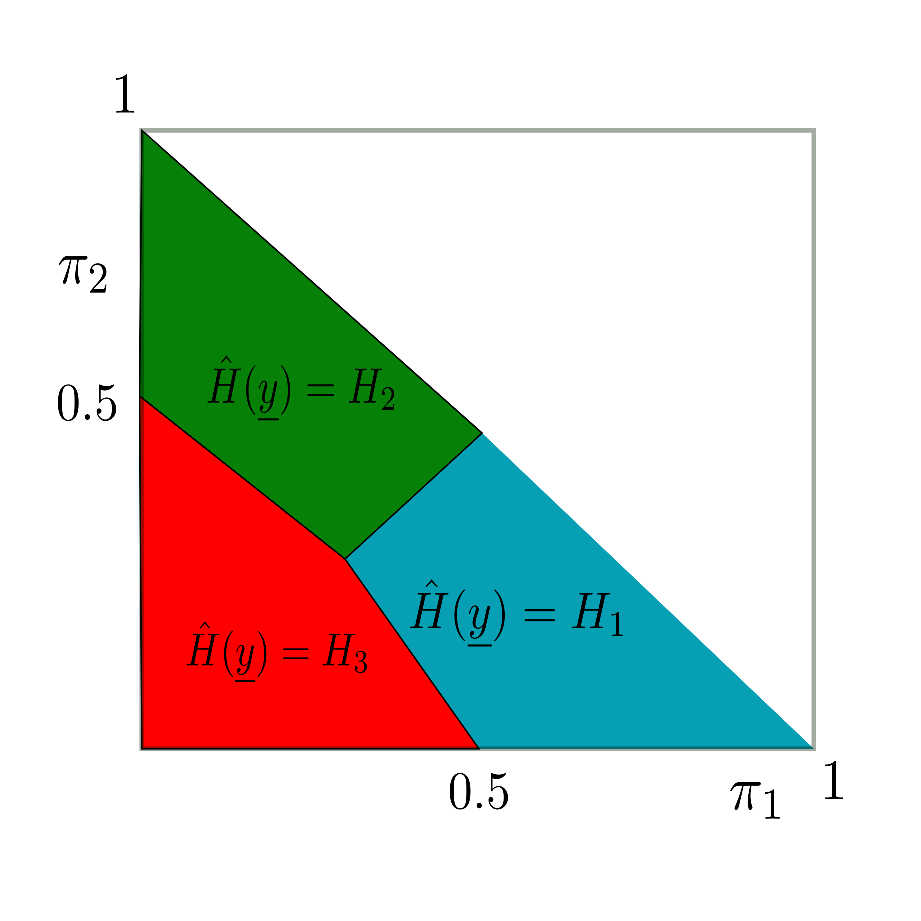
\includegraphics[width=7cm]{c3f1.eps}
    \caption{决策区域}\label{fig:c3f1}
    \end{figure}
    
    \end{enumerate}
    
  \item
    若$L_i(\urvy),i=2,3$已知,则
    \[
       \frac{p_{\underline{y}|\mathsf{H}}(\underline{y}|H_2)}
       {p_{\underline{y}|\mathsf{H}}(\underline{y}|H_3)}=\frac{L_2(\underline{y})}
       {L_3(\underline{y})}
    \]
    另一方面,因为$H_i$的先验均相等,基于后验概率的$\underline{\pi}(\underline{y})$正比于
    \[
    \begin{bmatrix}
    p_{\underline{y}|\mathsf{H}}(\underline{y}|H_1)\\
    p_{\underline{y}|\mathsf{H}}(\underline{y}|H_2)\\
    p_{\underline{y}|\mathsf{H}}(\underline{y}|H_3)
    \end{bmatrix}
    \]
    所以最优决策准则可以用$L_i(\underline{y}),i=2,3$给出。
    \begin{align*}
    p_{\underline{y}|\mathsf{H}}(\underline{y}|H_1)=\frac{\exp(-\frac{(y_1-1)^2+y_2^2+y_3^2}{2\sigma^2})}{\sqrt{2\pi}^3\sigma^3}\\    
    p_{\underline{y}|\mathsf{H}}(\underline{y}|H_2)=\frac{\exp(-\frac{y_1^2+(y_2-1)^2+y_3^2}{2\sigma^2})}{\sqrt{2\pi}^3\sigma^3}\\    
    p_{\underline{y}|\mathsf{H}}(\underline{y}|H_3)=\frac{\exp(-\frac{y_1^2+y_2^2+(y_3-1)^2}{2\sigma^2})}{\sqrt{2\pi}^3\sigma^3}
    \end{align*}
    因此
    \begin{align*}
    L_2(\underline{y})=\exp(-\frac{\ell_2(\underline{y})}{\sigma^2})\\
    L_3(\underline{y})=\exp(-\frac{\ell_3(\underline{y})}{\sigma^2})
    \end{align*}
    
  \end{enumerate}  
  \item  
  \begin{enumerate}[label=(\alph*)]
    \item 
    根据Bayes风险最小的准则,$\hat{x}=-1$当后验概率满足
    \[
     p_{x|\underline{\hat{x}}}(x=1| \underline{\hat{x}}) \leq 
     p_{x|\underline{\hat{x}}}(x=-1| \underline{\hat{x}})
    \]
    否则取$\hat{x}=1$
    由$P_{\mathsf{x}}(1)=P_{\mathsf{x}}(-1)=1/2$,得
    \[
     p_{\underline{\hat{x}}|x}(\underline{\hat{x}}|x=1) \leq 
     p_{\underline{\hat{x}}|x}(\underline{\hat{x}}|x=-1)
    \]
    记
    \[
    \phi(k)=\begin{cases}
    \frac{3}{4} & k>0 \\
    \frac{1}{4} & k\leq 0
    \end{cases}
    \]    
    则由独立性假设
    \begin{align*}
    p_{\underline{\hat{x}}|x}(\underline{\hat{x}}|x=1)
    = & \prod_{i=1}^n p_{\hat{x_i}|x}(\hat{x_i}|x=1) \\
    = & \prod_{i=1}^n \phi(\hat{x_i})
    \end{align*}
    同理
    \[
    p_{\underline{\hat{x}}|x}(\underline{\hat{x}}|x=-1)=\prod_{i=1}^{n} \phi(-\hat{x_i})
    \]
    因此最小错误概率的判决准则是:
    $$
    \left(\frac{3}{4}\right)^{\sum_i 1_{\hat{x}_i=1}}\left(\frac{1}{4}\right)^{\sum_i 1_{\hat{x}_i=-1}}\mathop{\gtreqless}_{\hat{x}=-1}^{\hat{x}=1} 
    \left(\frac{3}{4}\right)^{\sum_i 1_{\hat{x}_i=-1}}\left(\frac{1}{4}\right)^{\sum_i 1_{\hat{x}_i=1}}
    $$
    \item 若 $\hat{x}_1(y_1)=1(H_1)$, 期望损失为:
    \begin{align*}
    \tilde{\varphi}(H_1,y_1)=&C(1,1,1)p_{\mathsf{H},\hat{x}_2|\rvy}(\hat{x}_2=1,\rvx=1|y_1)
    +C(1,1,-1)p_{\mathsf{H},\hat{x}_2|\rvy}(\hat{x}_2=1,\rvx=-1|y_1)\\
    +&
    C(1,-1,1)p_{\mathsf{H},\hat{x}_2|\rvy}(\hat{x}_2=-1,\rvx=1|y_1)+
    C(1,-1,-1)p_{\mathsf{H},\hat{x}_2|\rvy}(\hat{x}_2=-1,\rvx=-1|y_1)\\
    \Rightarrow \tilde{\varphi}(H_1,y_1)p_{\rvy_1}(y_1) =& C(1,1,1)p_{\rvx}(\rvx=1)p_{\hat{x}_2|\rvx}(\hat{x}_2=1|\rvx=1)p_{\rvy_1|\rvx}(y_1|\rvx=1)\\
    +&C(1,1,-1)p_{\rvx}(\rvx=-1)p_{\hat{x}_2|\rvx}(\hat{x}_2=1|\rvx=-1)p_{\rvy_1|\rvx}(y_1|\rvx=-1)\\
    +&C(1,-1,1)p_{\rvx}(\rvx=1)p_{\hat{x}_2|\rvx}(\hat{x}_2=-1|\rvx=1)p_{\rvy_1|\rvx}(y_1|\rvx=1)\\
    +&C(1,-1,-1)p_{\rvx}(\rvx=-1)p_{\hat{x}_2|\rvx}(\hat{x}_2=-1|\rvx=-1)p_{\rvy_1|\rvx}(y_1|\rvx=-1)
    \end{align*}
    同理给出$\hat{x}_1(y_1)=-1(H_0)$, 期望损失$\tilde{\varphi}(H_0,y_1)$满足:
    \begin{align*}
    \tilde{\varphi}(H_0,y_1)p_{\rvy_1}(y_1)=& C(-1,1,1)p_{\rvx}(\rvx=1)p_{\hat{x}_2|\rvx}(\hat{x}_2=1|\rvx=1)p_{\rvy_1|\rvx}(y_1|\rvx=1)\\
    +&C(-1,1,-1)p_{\rvx}(\rvx=-1)p_{\hat{x}_2|\rvx}(\hat{x}_2=1|\rvx=-1)p_{\rvy_1|\rvx}(y_1|\rvx=-1)\\
    +&C(-1,-1,1)p_{\rvx}(\rvx=1)p_{\hat{x}_2|\rvx}(\hat{x}_2=-1|\rvx=1)p_{\rvy_1|\rvx}(y_1|\rvx=1)\\
    +&C(-1,-1,-1)p_{\rvx}(\rvx=-1)p_{\hat{x}_2|\rvx}(\hat{x}_2=-1|\rvx=-1)p_{\rvy_1|\rvx}(y_1|\rvx=-1)
    \end{align*}
    当$\tilde{\varphi}(H_0,y_1)\leq \tilde{\varphi}(H_1,y_1)$时接受$H_0$,
    得 $\gamma_2 p_{\rvy_1|\rvx}(y_1|\rvx=1) \leq \gamma_3 p_{\rvy_1|\rvx}(y_1| \rvx=-1)$
    其中
    \begin{align*}
    \gamma_2=& C(-1,1,1)p_{\rvx}(\rvx=1)p_{\hat{x}_2|\rvx}(\hat{x}_2=1|\rvx=1)
    +C(-1,-1,1)p_{\rvx}(\rvx=1)p_{\hat{x}_2|\rvx}(\hat{x}_2=-1|\rvx=1)\\
    -&C(1,1,1)p_{\rvx}(\rvx=1)p_{\hat{x}_2|\rvx}(\hat{x}_2=1|\rvx=1)
    -C(1,-1,1)p_{\rvx}(\rvx=1)p_{\hat{x}_2|\rvx}(\hat{x}_2=-1|\rvx=1)
    \end{align*}
    \begin{align*}
    \gamma_3=& C(-1,1,-1)p_{\rvx}(\rvx=-1)p_{\hat{x}_2|\rvx}(\hat{x}_2=1|\rvx=-1)\\
    +&C(-1,-1,-1)p_{\rvx}(\rvx=-1)p_{\hat{x}_2|\rvx}(\hat{x}_2=-1|\rvx=-1)\\
    -&C(1,1,-1)p_{\rvx}(\rvx=-1)p_{\hat{x}_2|\rvx}(\hat{x}_2=1|\rvx=-1)
    -C(1,-1,-1)p_{\rvx}(\rvx=-1)p_{\hat{x}_2|\rvx}(\hat{x}_2=-1|\rvx=-1)
    \end{align*}
    
    根据$C(\hat{x}_1,\hat{x}_2,x)$的性质,
    $C(-1,1,1)>C(1,1,1),C(-1,-1,1)>C(1,-1,1)$,所以
    $\gamma_2>0$,因此
    \[
     \frac{p_{\rvy_1|\rvx}(y_1|\rvx=1)}{p_{\rvy_1|\rvx}(y_1| \rvx=-1)} \leq \frac{\gamma_3}{\gamma_2} \defas \gamma_1
    \]
    另解:
    \begin{align*}
      \bar{R} = & \sum_{x_1,x_2,\tilde{x}=-1,1} C(x_1,x_2,\tilde{x}) P(\hat{\rvx}_1 =x_1,\hat{\rvx}_2 = x_2 , \rvx = \tilde{x}) \\
              = & \sum_{x_1,x_2,\tilde{x}=-1,1} C(x_1,x_2,\tilde{x}) P_{\rvx}(\tilde{x})P_{\hat{\rvx}_1|\rvx}(x_1 | \tilde{x})P_{\hat{\rvx}_2|\rvx}(x_2 |\tilde{x}) \\
              = & \sum_{x_2,\tilde{x}=-1,1} C(1,x_2,\tilde{x}) P_{\rvx}(\tilde{x})P_{\hat{\rvx}_2|\rvx}(x_2 | \tilde{x})\int_{y_1\in \mathcal{Y}_1} p_{\rvy_1|\rvx}(y_1|\tilde{x})dy_1 \\
             + & \sum_{x_2,\tilde{x}=-1,1} C(-1,x_2,\tilde{x}) P_{\rvx}(\tilde{x})P_{\hat{\rvx}_2|\rvx}(x_2 | \tilde{x})\int_{y_1\in \mathcal{Y}_0} p_{\rvy_1|\rvx}(y_1|\tilde{x})dy_1 \\
              = & \sum_{x_2,\tilde{x}=-1,1} C(-1,x_2,\tilde{x}) P_{\rvx}(\tilde{x})P_{\hat{\rvx}_2|\rvx}(x_2 | \tilde{x}),\mathcal{Y}_1 \cup \mathcal{Y}_0=\mathbb{R} \\
             + &  \int_{y_1\in \mathcal{Y}_1} \sum_{x_2,\tilde{x}=-1,1}\left(C(1,x_2,\tilde{x})-C(-1,x_2,\tilde{x})\right)P_{\hat{\rvx}_2|\rvx}(x_2 | \tilde{x}) P_{\rvx}(\tilde{x})p_{\rvy_1|\rvx}(y_1|\tilde{x})dy_1 \\
    \end{align*}
    因此
\begin{align*}
y_1\in \mathcal{Y}_1 \iff & \sum_{x_2,\tilde{x}=-1,1}\left(C(1,x_2,\tilde{x})-C(-1,x_2,\tilde{x})\right)P_{\hat{\rvx}_2|\rvx}(x_2 | \tilde{x}) P_{\rvx}(\tilde{x})p_{\rvy_1|\rvx}(y_1|\tilde{x}) < 0 \\
\iff & \sum_{x_2=-1,1}\left(C(1,x_2,1)-C(-1,x_2,1)\right) P_{\hat{\rvx}_2|\rvx}(x_2 | 1)P_{\rvx}(1)p_{\rvy_1|\rvx}(y_1|1) \\
< & \sum_{x_2=-1,1}\left(C(-1,x_2,-1)-C(1,x_2,-1)\right) P_{\hat{\rvx}_2|\rvx}(x_2 | -1)P_{\rvx}(-1)p_{\rvy_1|\rvx}(y_1|-1) \\
\iff  & \frac{p_{\rvy_1|\rvx}(y_1|1)}{p_{\rvy_1|\rvx}(y_1|-1)} > \gamma_1 \\
\gamma_1 = & \frac{P_{\rvx}(-1)\sum_{x_2=-1,1}\left(C(-1,x_2,-1)-C(1,x_2,-1)\right) P_{\hat{\rvx}_2|\rvx}(x_2 | -1)}{P_{\rvx}(1)\sum_{x_2=-1,1}\left(C(1,x_2,1)-C(-1,x_2,1)\right) P_{\hat{\rvx}_2|\rvx}(x_2 | 1)}
\end{align*}    
    \item 由对称性,根据(b)中的结果,可得最优的决策准则$\hat{x}_2^*(\dot)$是如下形式的
    似然比检验:
    \[
      \frac{p_{\rvy_2|\rvx}(y_2|\rvx=1)}{p_{\rvy_2|\rvx}(y_2| \rvx=-1)} \mathop{\gtreqless}_{\hat{x}_2(y_1) = 1}^{\hat{x}_2(y_1) = -1} \frac{\gamma'_2}{\gamma'_3} \defas \gamma'_1
    \]
    其中
    \begin{align*}
    \gamma'_2=& C(1,-1,1)p_{\rvx}(\rvx=1)p_{\hat{x}_1|\rvx}(\hat{x}_1=1|\rvx=1)
    +C(-1,-1,1)p_{\rvx}(\rvx=1)p_{\hat{x}_1|\rvx}(\hat{x}_1=-1|\rvx=1)\\
    -&C(1,1,1)p_{\rvx}(\rvx=1)p_{\hat{x}_1|\rvx}(\hat{x}_1=1|\rvx=1)
    -C(-1,1,1)p_{\rvx}(\rvx=1)p_{\hat{x}_1|\rvx}(\hat{x}_1=-1|\rvx=1)
    \end{align*}
    \begin{align*}
    \gamma'_3=& C(1,-1,-1)p_{\rvx}(\rvx=-1)p_{\hat{x}_1|\rvx}(\hat{x}_1=1|\rvx=-1)\\
    +&C(-1,-1,-1)p_{\rvx}(\rvx=-1)p_{\hat{x}_1|\rvx}(\hat{x}_1=-1|\rvx=-1)\\
    -&C(1,1,-1)p_{\rvx}(\rvx=-1)p_{\hat{x}_1|\rvx}(\hat{x}_1=1|\rvx=-1)
    -C(-1,1,-1)p_{\rvx}(\rvx=-1)p_{\hat{x}_1|\rvx}(\hat{x}_1=-1|\rvx=-1)
    \end{align*}
    \item (b)中$\gamma_2,\gamma_3$可化简为:
    \begin{align*}
    \gamma_2 =& p_{\rvx}(\rvx=1)p_{\hat{x}_2|\rvx}(\hat{x}_2=1|\rvx=1)
    +Lp_{\rvx}(\rvx=1)p_{\hat{x}_2|\rvx}(\hat{x}_2=-1|\rvx=1)\\    
    -&p_{\rvx}(\rvx=1)p_{\hat{x}_2|\rvx}(\hat{x}_2=-1|\rvx=1)\\
    =&p_{\rvx}(\rvx=1)(1+(L-2)p_{\hat{x}_2|\rvx}(\hat{x}_2=-1|\rvx=1))    
    \end{align*}
    \begin{align*}
    \gamma_3 =&p_{\rvx}(\rvx=-1)p_{\hat{x}_2|\rvx}(\hat{x}_2=1|\rvx=-1)\\    
    -&Lp_{\rvx}(\rvx=-1)p_{\hat{x}_2|\rvx}(\hat{x}_2=1|\rvx=-1)
    -p_{\rvx}(\rvx=-1)p_{\hat{x}_2|\rvx}(\hat{x}_2=-1|\rvx=-1)\\
    =&-p_{\rvx}(\rvx=-1)(1+(L-2)p_{\hat{x}_2|\rvx}(\hat{x}_2=1|\rvx=-1))
    \end{align*}
    因此,当$L=2$时,$\gamma=-\frac{p_{\rvx}(\rvx=1)}{p_{\rvx}(\rvx=-1)}$,与$\hat{x}_2$无关;
    同理求出$\gamma'=\gamma$.
    \end{enumerate}
  \item 上机作业  
  \item Thanks to 陆石, who gives me this template.
  

  \end{enumerate}

\end{document}
\begin{equation}
\end{equation}

%%% Local Variables:
%%% mode: late\rvx
%%% TeX-master: t
%%% End:
